\chapter{Super-cells and nanoislands}
\section{Simple}
This is the simplest super-cell to implement, it is just a n-replication of the unit cell along the lattice vectors.
%~~~~~~~~~~~~~~~~~~~~~~~~~~ FIGURE ~~~~~~~~~~~~~~~~~~~~~~~~~%
\begin{figure}[h!]
\centering
   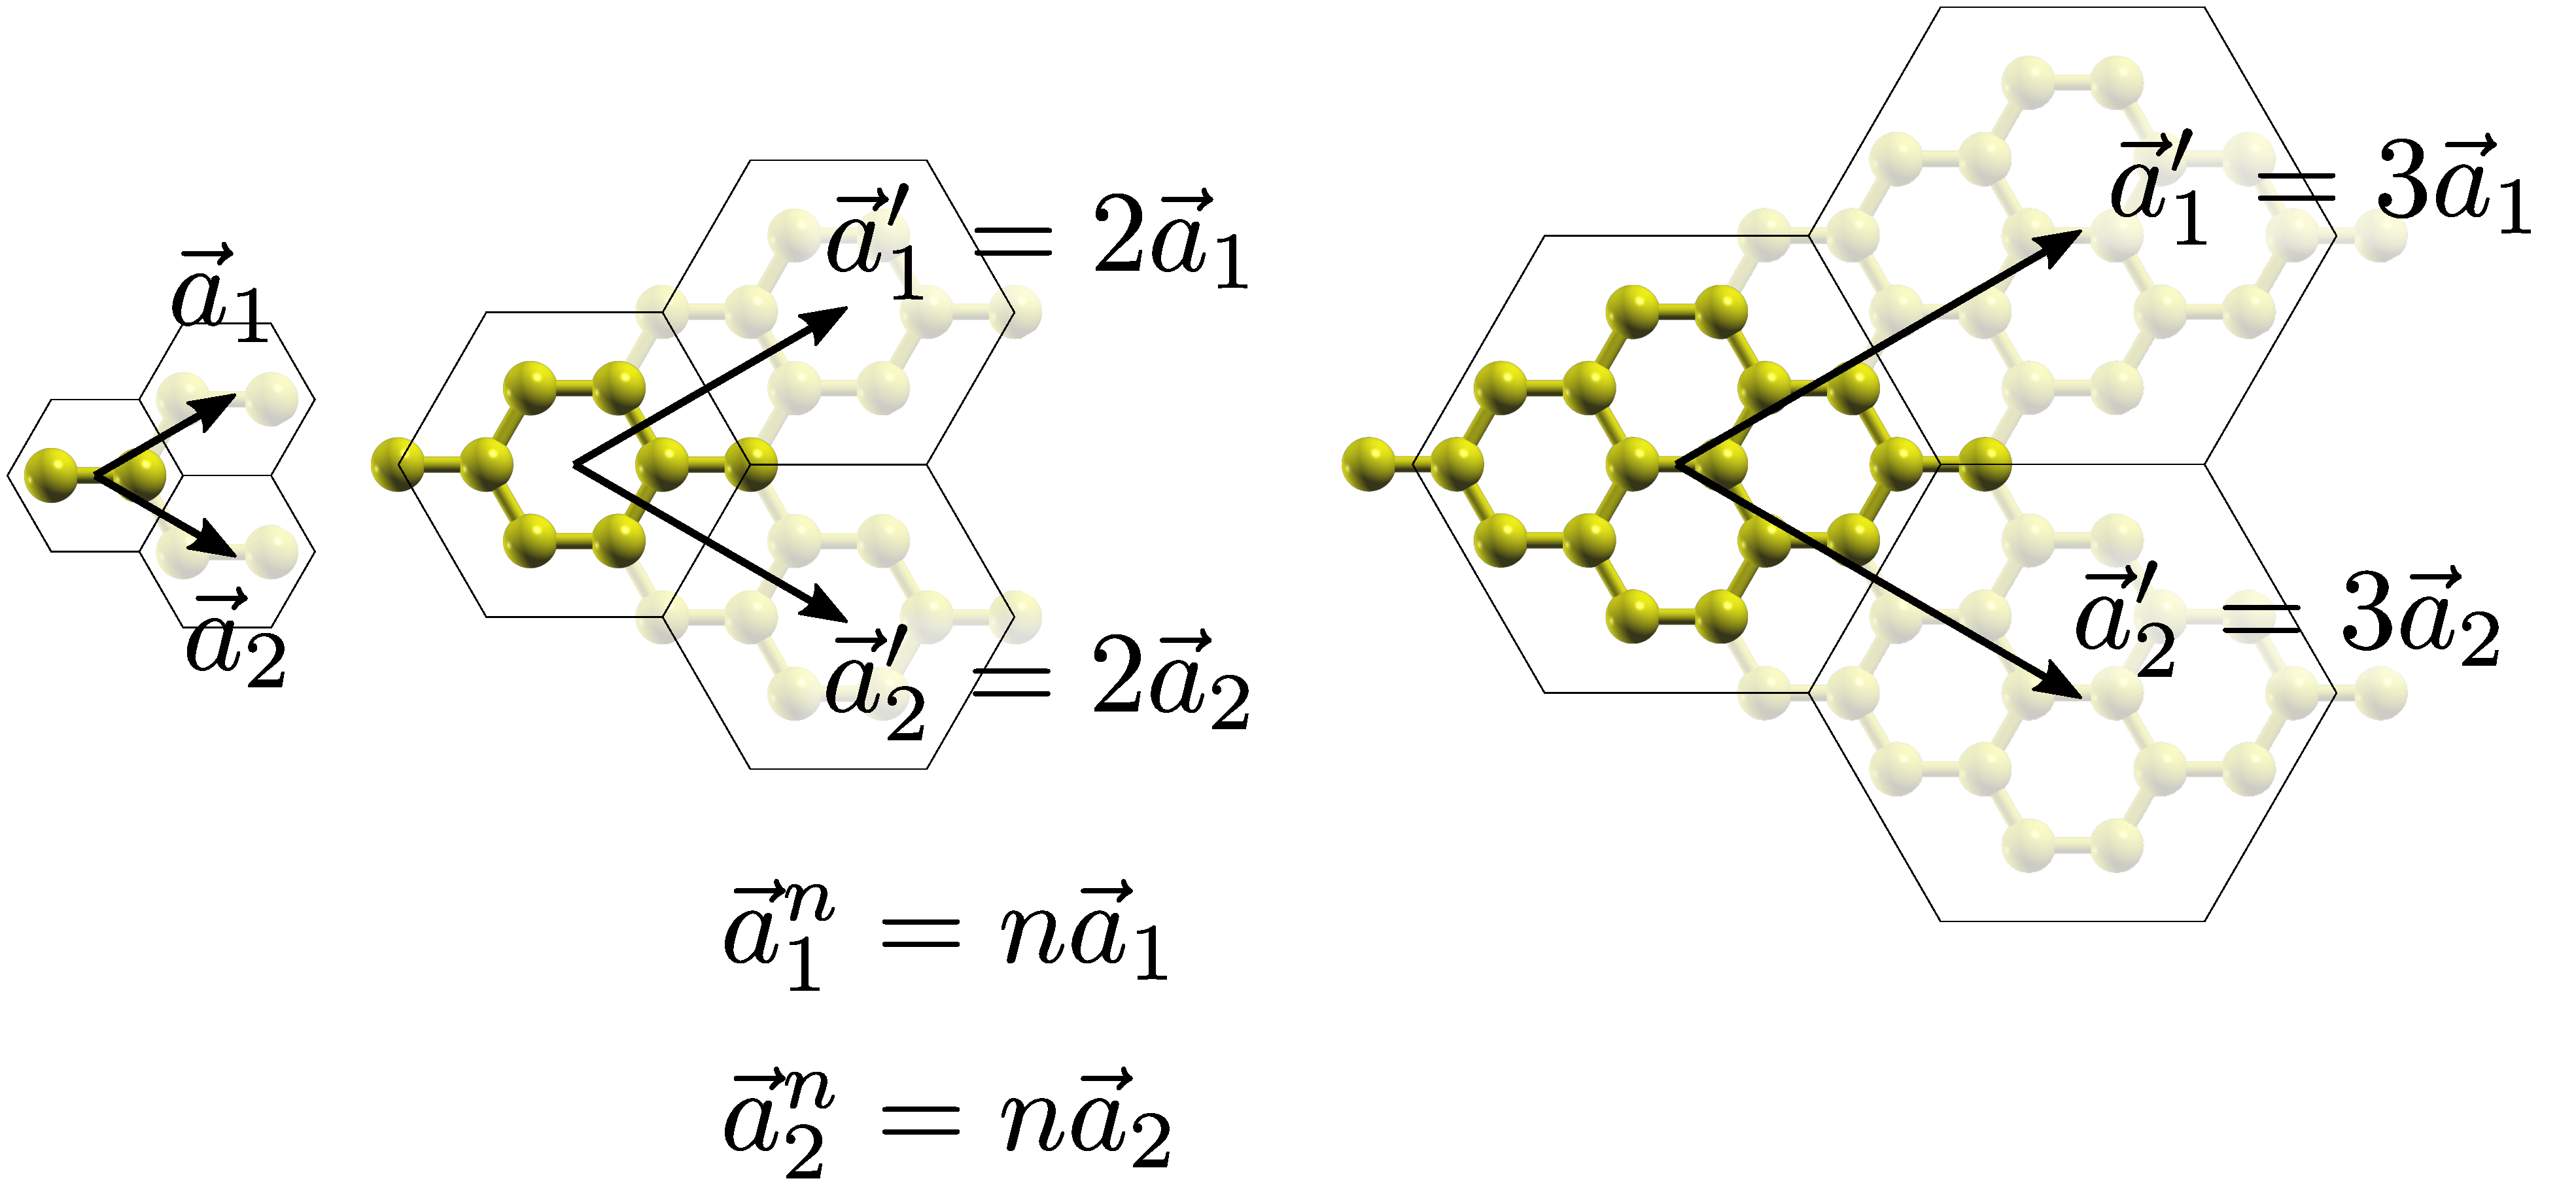
\includegraphics[width=0.8\textwidth]{appendix/figures/cells_simple.pdf}
\vspace{-5pt}
\caption{Caption}
\label{simple_islands}
\end{figure}
\FloatBarrier
%~~~~~~~~~~~~~~~~~~~~~~~~~~~~~~~~~~~~~~~~~~~~~~~~~~~~~~~~~~~%
\begin{equation}
   N = 2n^2
\end{equation}


\section{Armchair}
Taking a Benzene ring as building block, one can replicate it in the proper positions in order to generate bigger and bigger armchair islands. The process is not straight forward since it is not enough to replicate along the lattice vectors (or $\pm$ combinations of them), but rather 
%~~~~~~~~~~~~~~~~~~~~~~~~~~ FIGURE ~~~~~~~~~~~~~~~~~~~~~~~~~%
\begin{figure}[h!]
\centering
   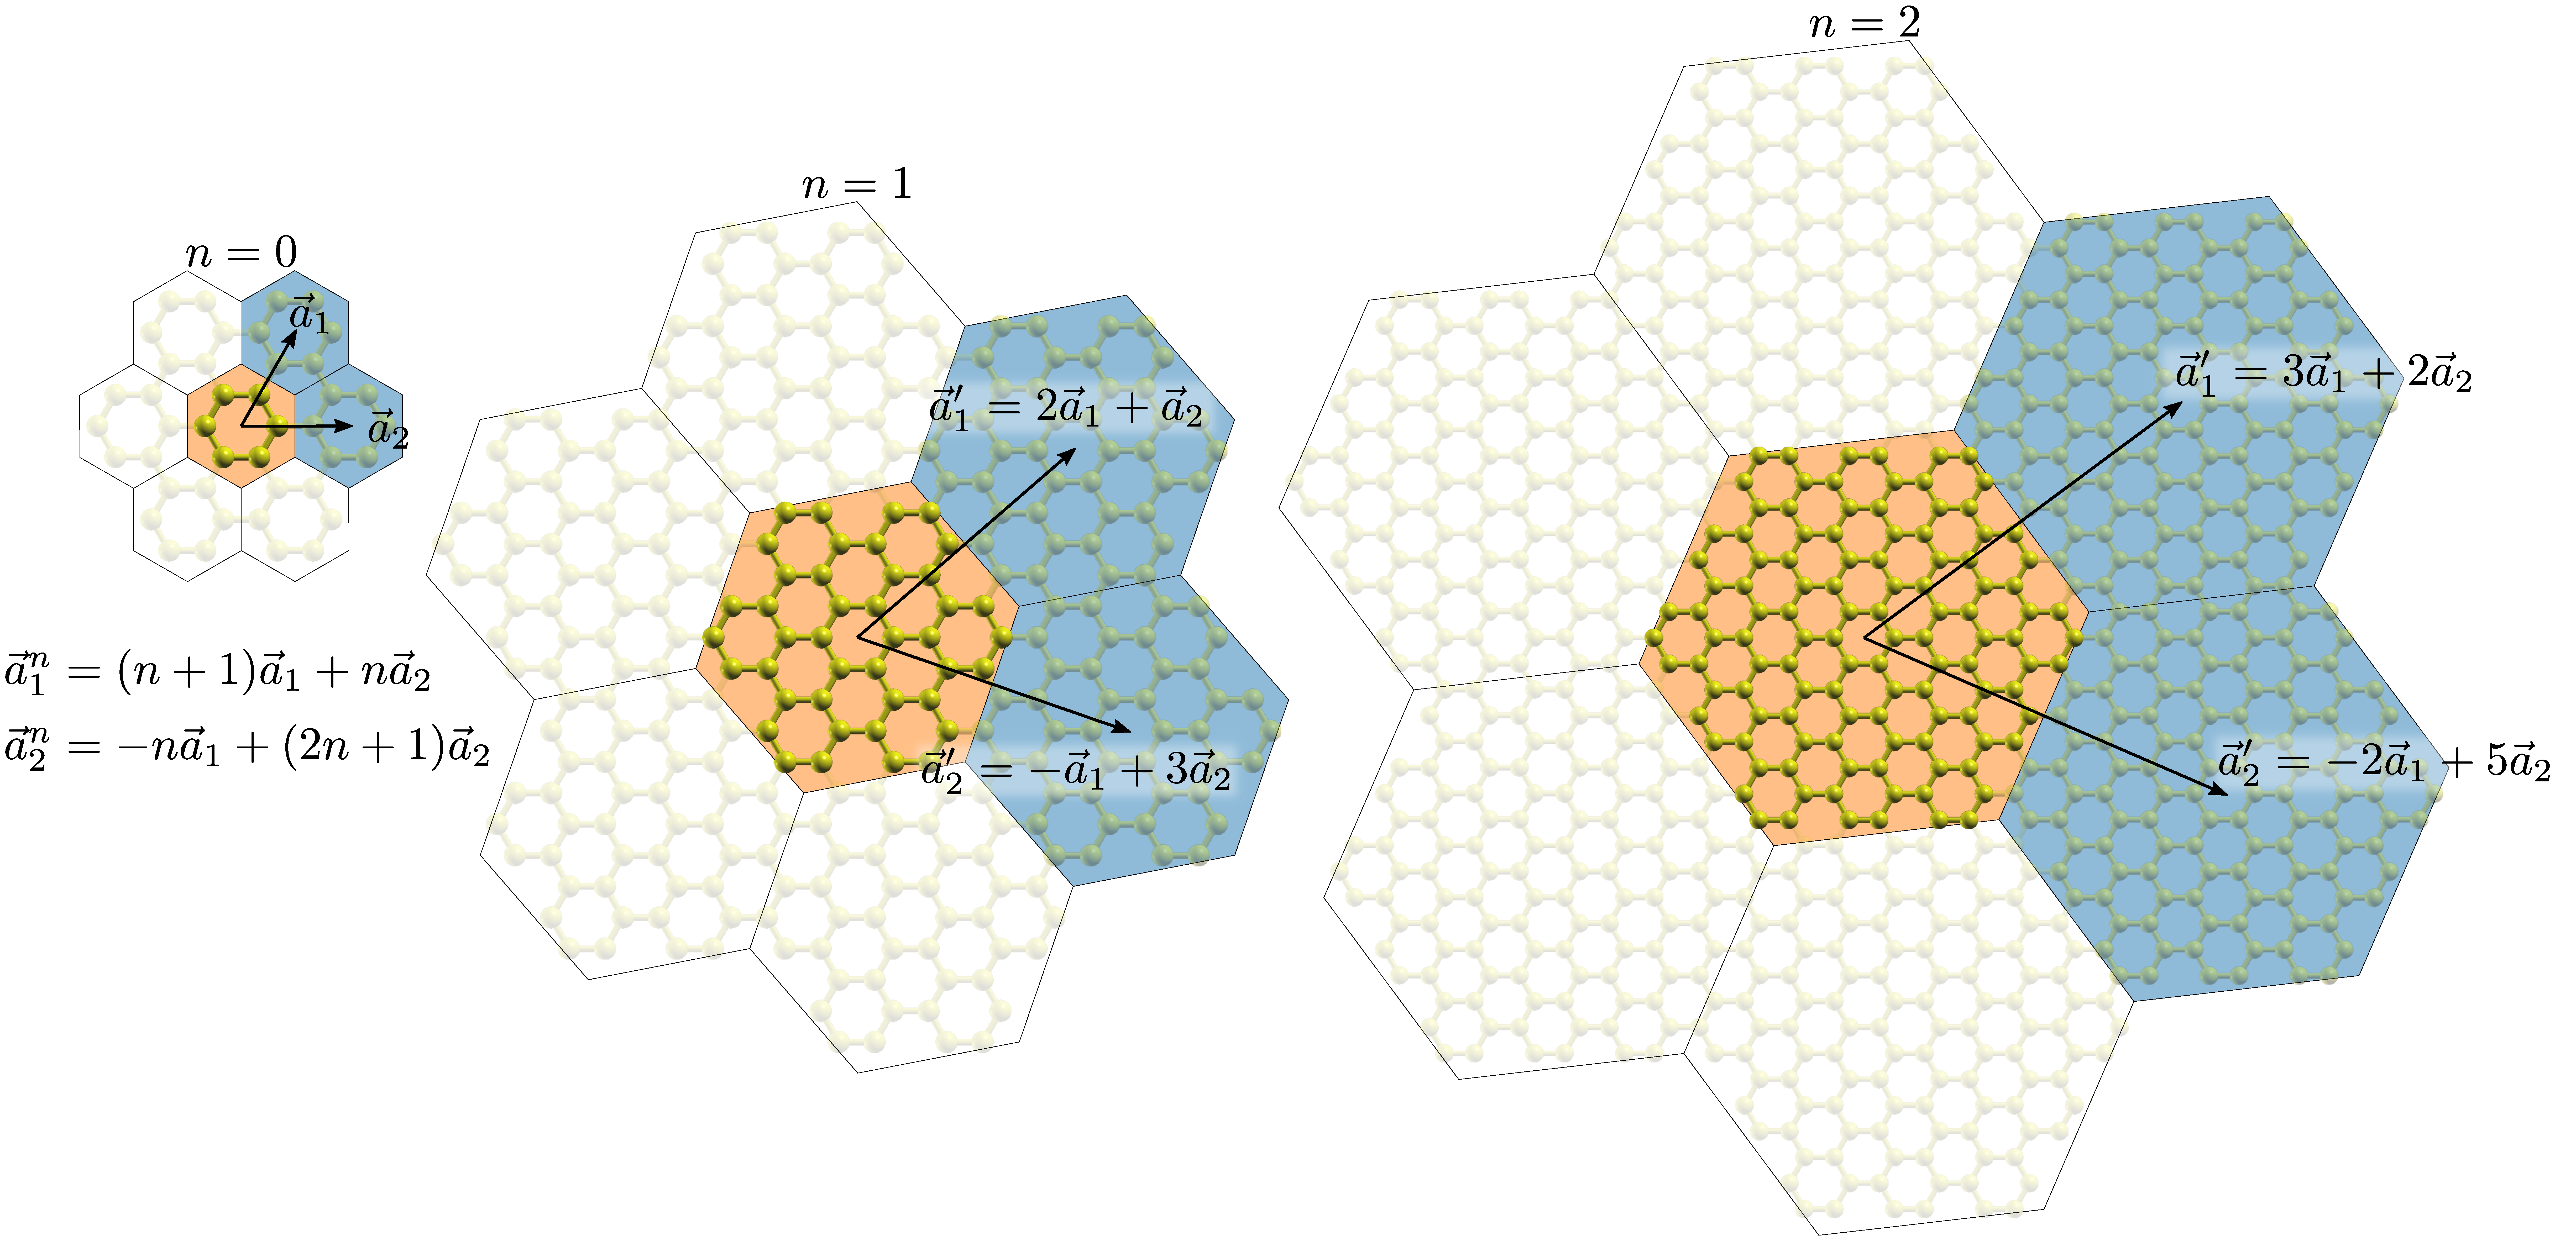
\includegraphics[width=0.8\textwidth]{appendix/figures/cells_ac.pdf}
\vspace{-5pt}
\caption{Three first supercells of armchair islands.}
\label{ac_islands}
\end{figure}
\FloatBarrier
%~~~~~~~~~~~~~~~~~~~~~~~~~~~~~~~~~~~~~~~~~~~~~~~~~~~~~~~~~~~%
\begin{equation}
   N = 6\cdot(3n^2-3n+1)
\end{equation}

This is how fast the number of carbon atoms grows for the different kind of islands.

%~~~~~~~~~~~~~~~~~~~~~~~~~~ FIGURE ~~~~~~~~~~~~~~~~~~~~~~~~~%
\begin{figure}[h!]
\centering
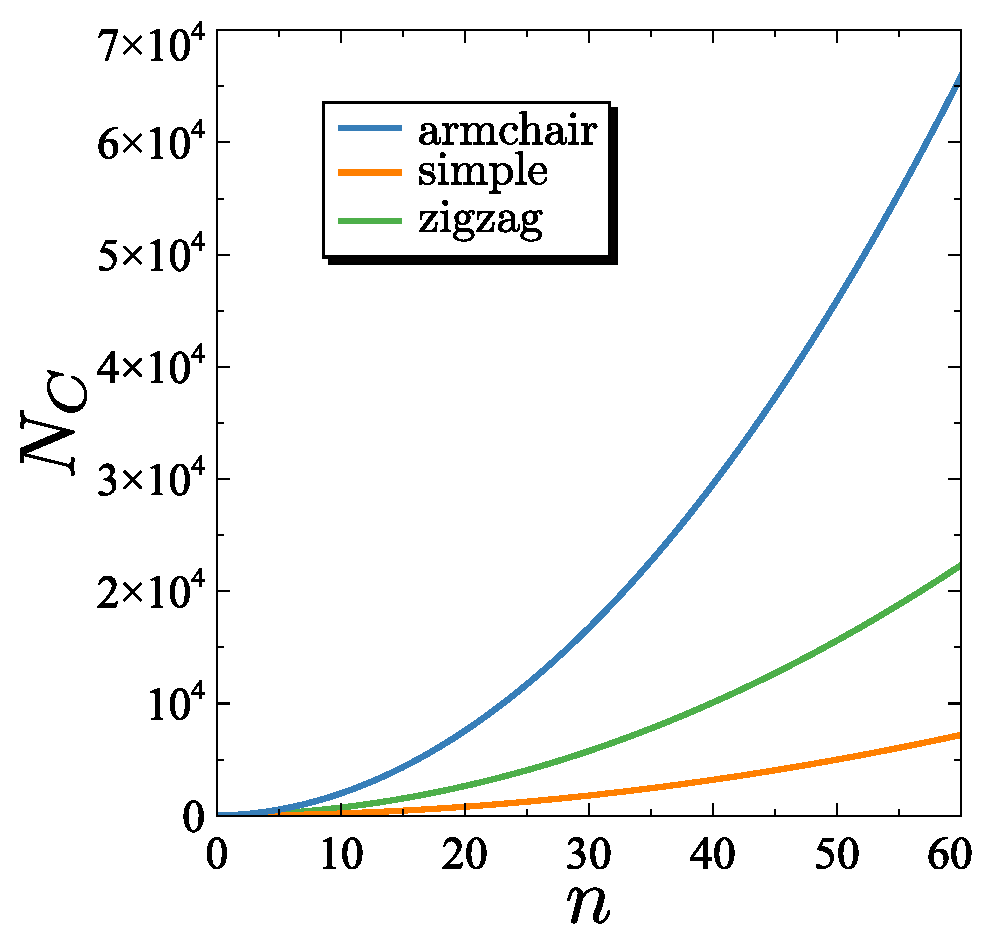
\includegraphics{appendix/figures/Nats.pdf}
\vspace{-5pt}
\caption{Evolution of the number of carbon atoms as the super-cell index grows. While the evolution is always quadratic, the armchair islands grows much faster than the rest of the models.}
\label{Nats}
\end{figure}
\FloatBarrier
%~~~~~~~~~~~~~~~~~~~~~~~~~~~~~~~~~~~~~~~~~~~~~~~~~~~~~~~~~~~%
